% 将本文件与 figures/ 文件夹复制到论文工程根目录。
% 主文档导言区需加载 graphicx；中文文档建议使用 XeLaTeX。
% 正文章号随主文档自动生成，本文件不修改章节计数器。
\subsection{数据观察与预处理}

附件1包含100条视频片段，分布于37个以原始视频编号命名的子文件夹中。本文以视频编号与片段编号的组合作为样本标识，将视频文件与 \texttt{label-100} 表中的英文转写、情感分值及类别标注逐一对应。通过核对样本清单并完整解码音视频流，确认100条样本均具有对应的视频与文本记录，且均可正常解码。在此基础上，统计片段时长与转写长度，并浏览全体样本的中点帧总览，观察原始数据的长度差异及画面内容。

视频片段的时长分布如图~\ref{fig:p1_duration}所示。按实际解码记录统计，视频片段时长为 $2.257$--$29.288\,\mathrm{s}$，平均时长为 $7.880\,\mathrm{s}$，中位数为 $6.722\,\mathrm{s}$。\footnote{本节时长取解码记录中视频终点与音频终点的较大者，以视频流起点为时间原点。该实测范围与题干所述的 $2.648$--$34.567\,\mathrm{s}$ 不一致，本文保留全部原始文件，并依据实际时间记录进行后续处理。}

给定转写的词数分布如图~\ref{fig:p1_transcript_length}所示。以英文字母词和数字串为计数单位，允许词内撇号，标点不单独计词，100条转写共包含1932个词，单条转写的词数为5--65，平均值为19.32，中位数为18。两幅分布图中的虚线分别表示时长与词数的中位数，其中词数按原文词统计，而非模型子词。

\begin{figure}[htp!]
    \centering
    \begin{minipage}[t]{0.48\linewidth}
        \vspace{0pt}
        \centering
        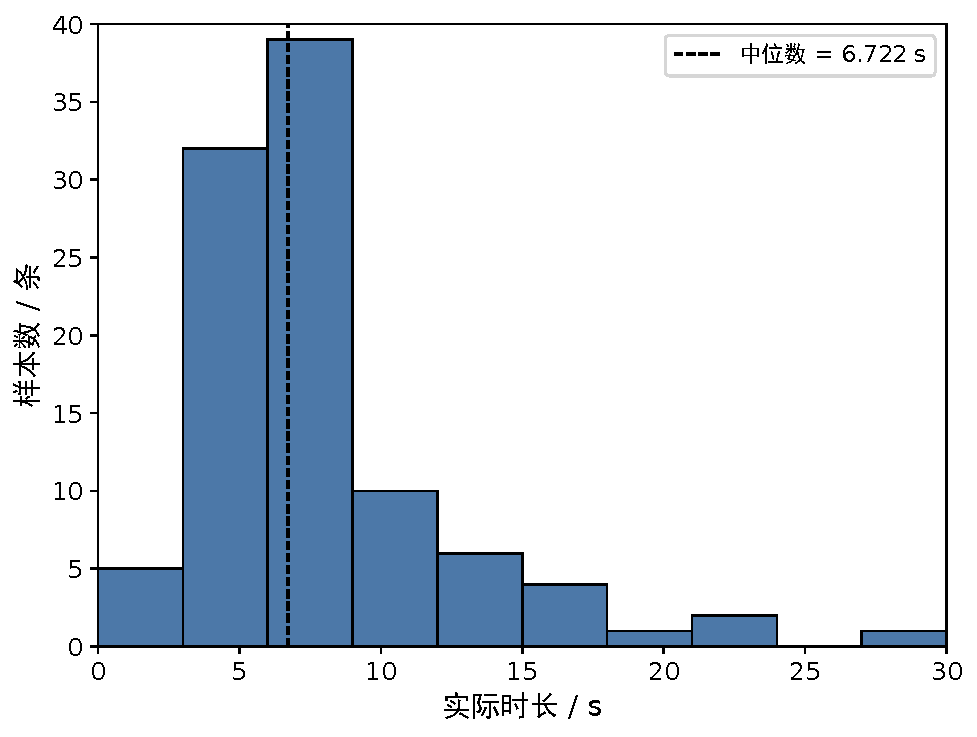
\includegraphics[width=\linewidth]{figures/fig_5_2_duration.pdf}
        \caption{原始视频片段的时长分布}
        \label{fig:p1_duration}
    \end{minipage}\hfill
    \begin{minipage}[t]{0.48\linewidth}
        \vspace{0pt}
        \centering
        
\includegraphics[width=\linewidth]{figures/fig_5_2_transcript_length.pdf}
        \caption{给定英文转写的词数分布}
        \label{fig:p1_transcript_length}
    \end{minipage}
\end{figure}

图~\ref{fig:p1_duration_words}进一步展示了片段时长与转写词数的联合分布，每个点对应一条视频片段。不同片段对应的序列规模存在差异，处理时需要保留各样本的实际长度，不能预设统一词数。

原始类别标注的构成如图~\ref{fig:p1_label_distribution}所示，按标签表原始 \texttt{annotation} 字段统计，正向、中性和负向样本分别为57条、25条和18条，柱上标注对应样本数。这些标注随样本保留，本问不据此训练特征提取模型。

\begin{figure}[htp!]
    \centering
    \begin{minipage}[t]{0.48\linewidth}
        \vspace{0pt}
        \centering
        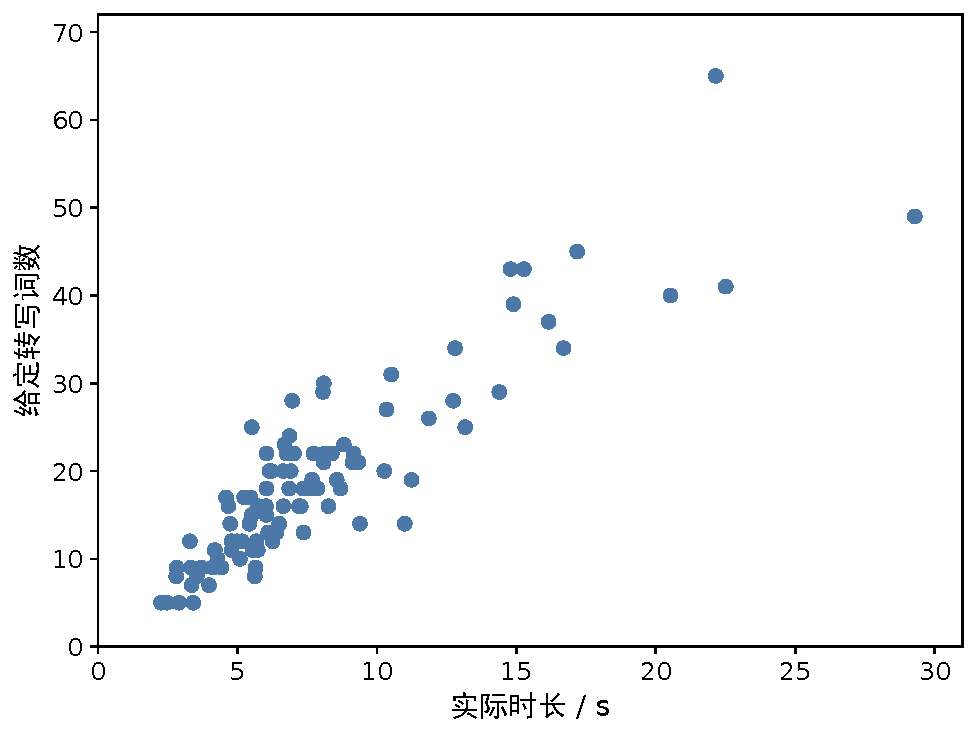
\includegraphics[width=\linewidth]{figures/fig_5_2_duration_words.pdf}
        \caption{片段时长与转写词数的联合分布}
        \label{fig:p1_duration_words}
    \end{minipage}\hfill
    \begin{minipage}[t]{0.48\linewidth}
        \vspace{0pt}
        \centering
        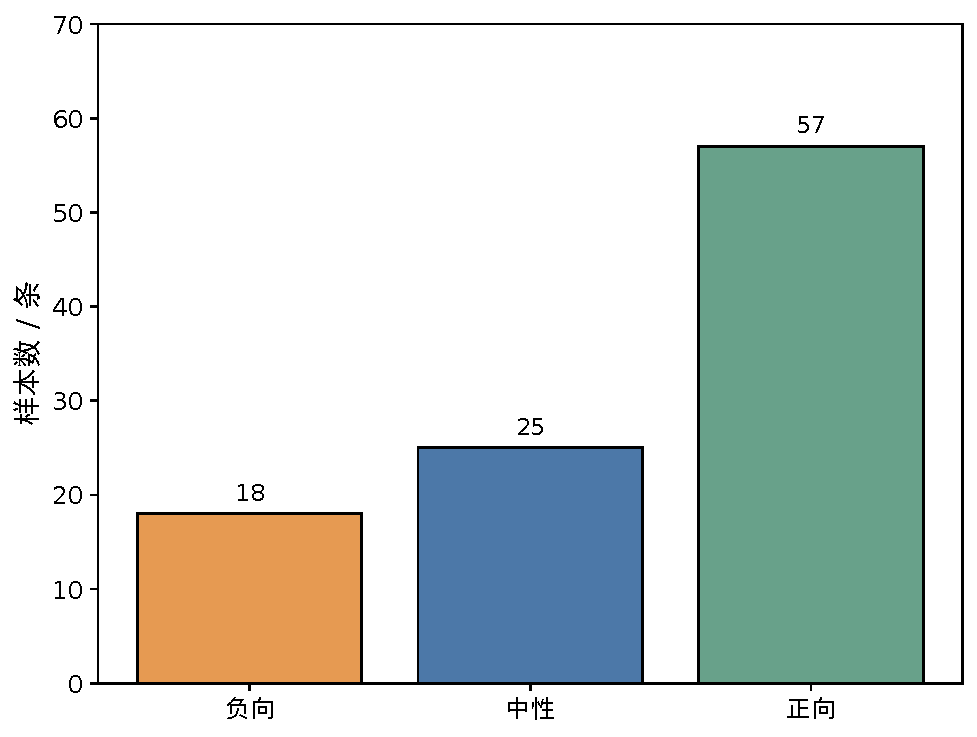
\includegraphics[width=\linewidth]{figures/fig_5_2_label_distribution.pdf}
        \caption{样本情感类别构成}
        \label{fig:p1_label_distribution}
    \end{minipage}
\end{figure}

原始画面的观察结果进一步表明，视频并非始终呈现清晰的人物面部。图~\ref{fig:p1_source_examples}展示了从中点帧总览中选取的六个内容不同的实例，既包括人物近景和人物与板书画面，也包括文字卡、器材、山体景观及图形画面。因此，视频帧的存在并不意味着能够提取有效的面部表情特征，后续需要分别记录视频帧的时间位置与面部观测有效性。这里的画面描述仅针对所展示的时刻，不据此判定整段视频是否包含人脸，也不将所选实例的比例作为全体数据的场景分布。

\begin{figure}[htbp]
    \centering
    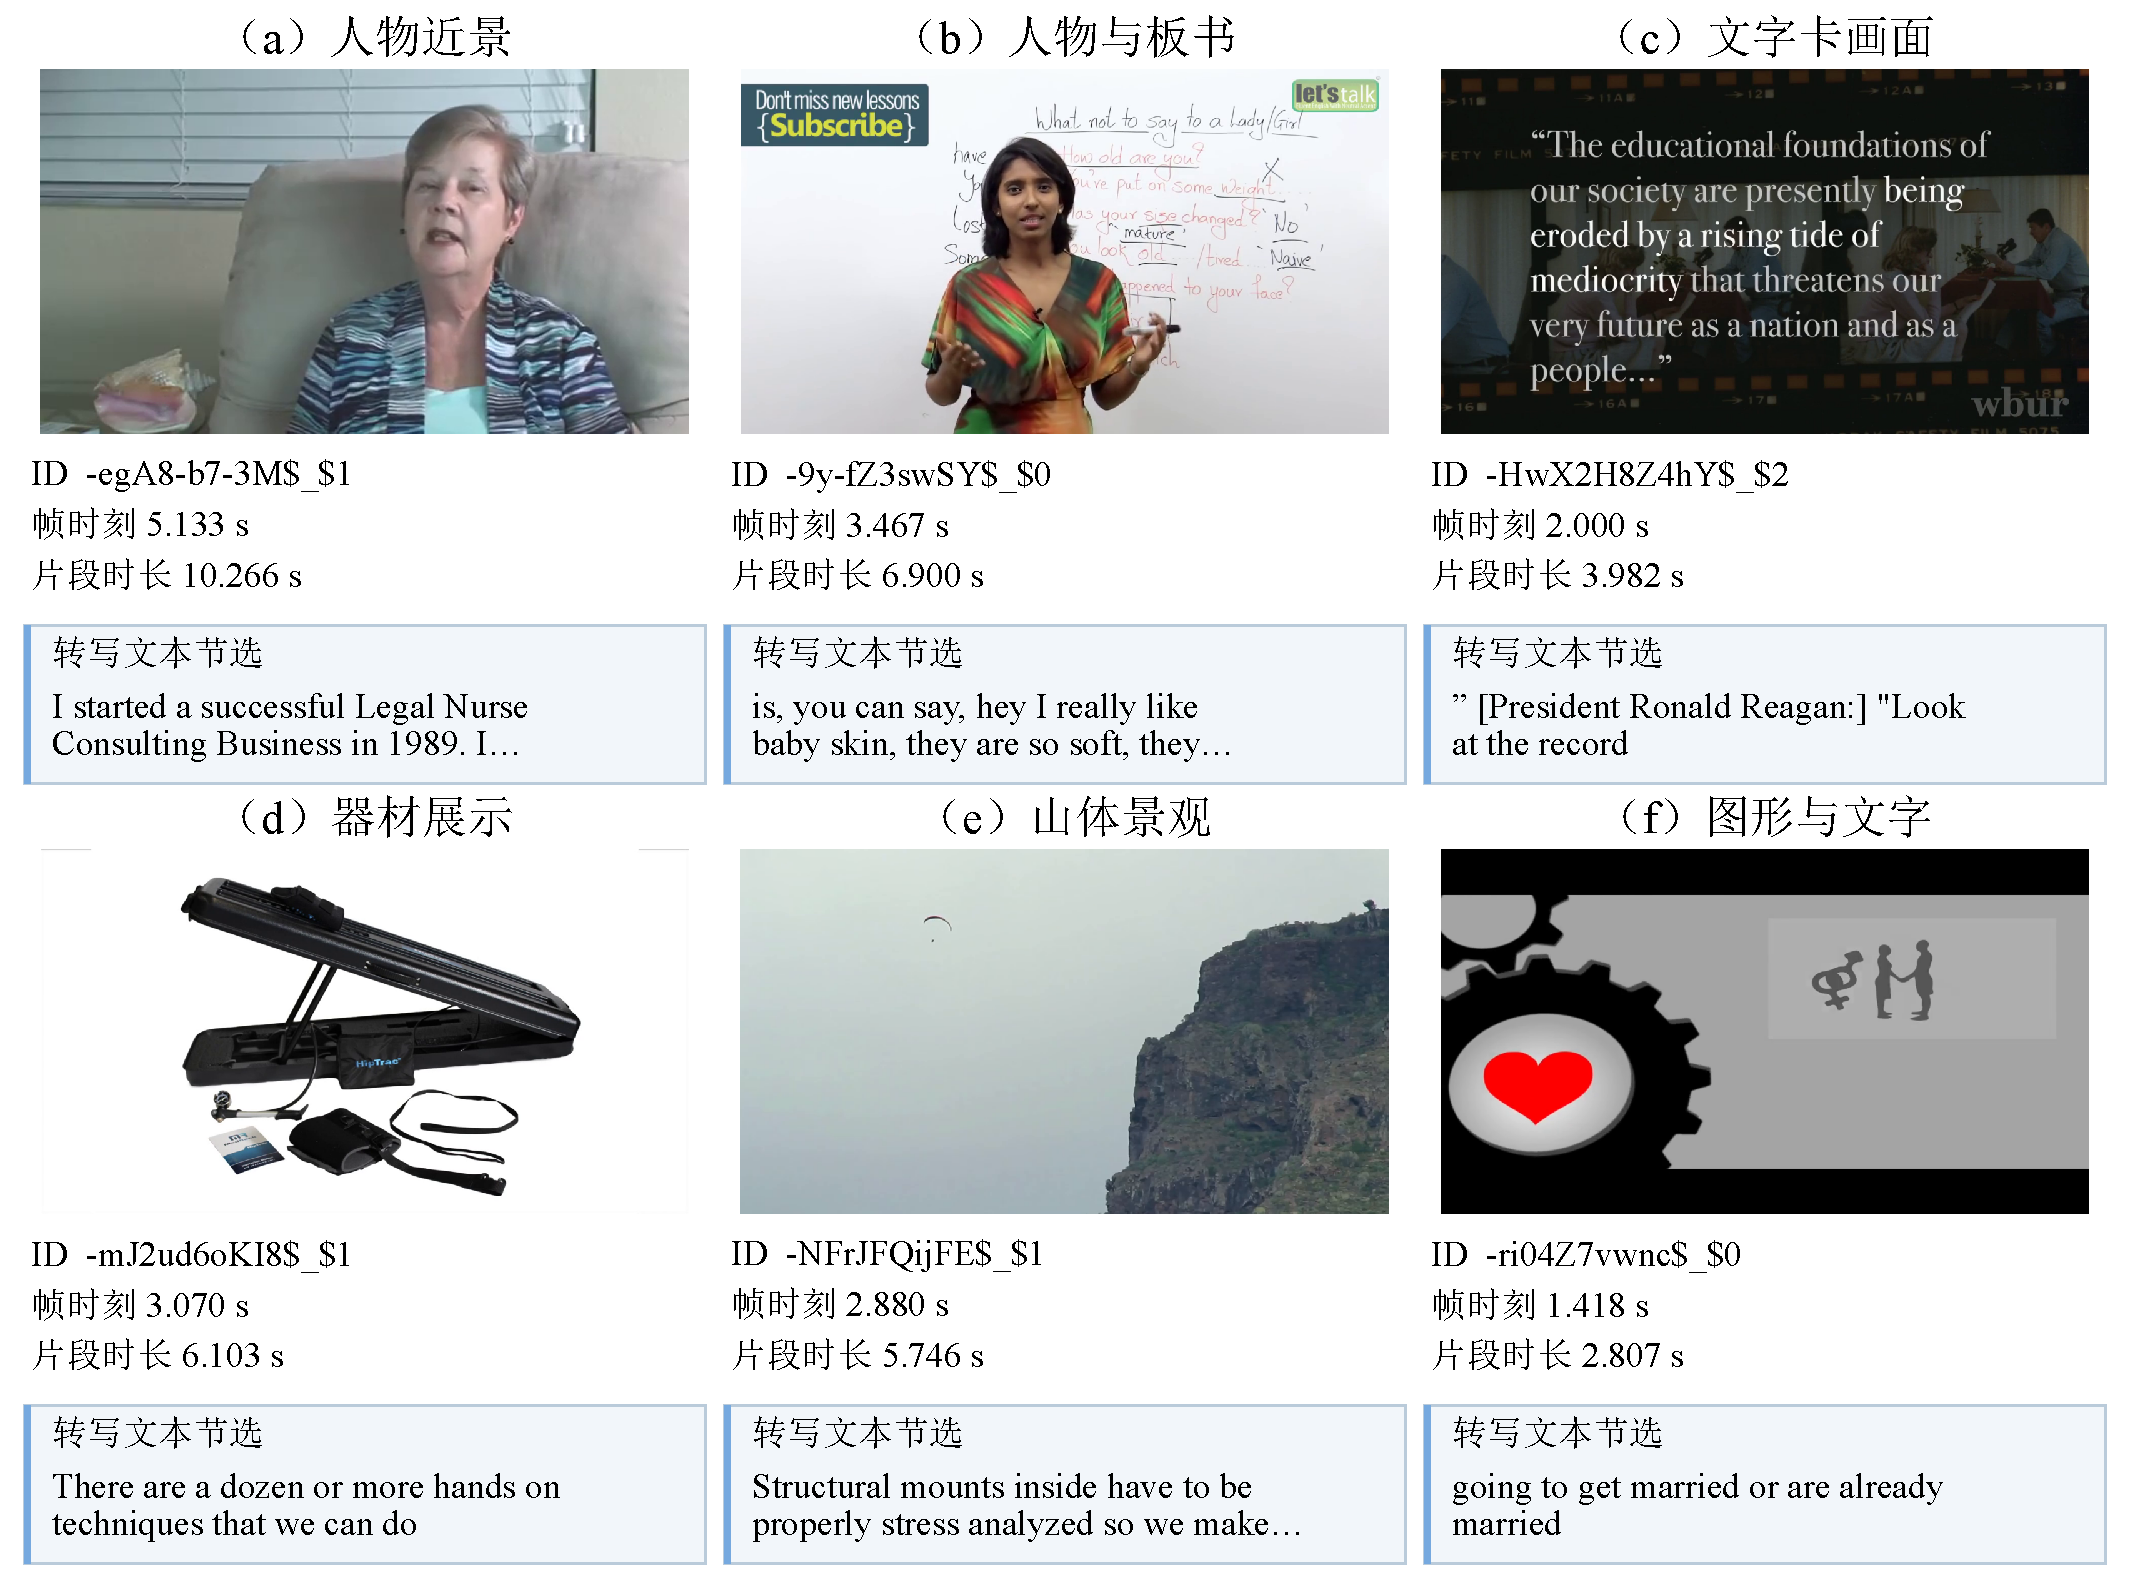
\includegraphics[width=\textwidth]{figures/fig_5_2_source_examples.pdf}
    \caption{原始视频画面与给定转写示例。各画面取自片段时长中点处或其后的首个实际视频帧，标注实际帧时刻、片段时长和样本编号。转写按标签表原文节选，省略部分以省略号表示；画面与整段转写的并列展示不表示二者已建立词级时间对应。}
    \label{fig:p1_source_examples}
\end{figure}

针对上述数据特点，本文首先保留完整转写及其标点，依据原文字符位置建立词索引，为后续词与子词之间的映射提供依据。原始转写中的数字、缩写及说明性文字均不直接删除或改写；用于声学对齐的文本规范化另行记录，避免改变原始文本内容。音频经解码后转换为采样率为 $16\,\mathrm{kHz}$ 的单声道信号，并保留其相对于视频起点的时间信息。视频则以约 $5\,\mathrm{Hz}$ 的目标频率抽取实际画面，保存所选帧的显示时间戳及原始帧索引，不以抽样序号代替实际时刻。

各样本按实际长度独立保存，不为获得统一序列长度而裁剪视频或截断转写。经过上述处理，原始文本位置、音频时间和视频帧时间均得到保留，为下一节分别提取三模态特征及随后建立词级时间对应关系提供基础。
